\section{Implementation}

\subsection{Build plan}

\blindtext

\subsection{Prototyping}

\subsubsection{DAW}

Our DAW prototype was constructed without the use of the Electron UI-building environment. This
decision was motivated by the belief that creating the Electron application encompassed two
separate problems: the first was to create a fully functioning script, the second was to port that
script into the Electron application. By building the prototype outside of Electron, we aimed for
faster progress and less bottlenecking of the workflow by dealing with one smaller problem at a
time. Additionally, this decision expedited the debugging process by removing the need to load
the full Electron application every time we wished to monitor the progress of the build. Instead,
we could simply locate the HTML file in out directory and open it in a browser with a single click.

The first step in constructing the DAW was to establish all of the static elements, which include
the piano roll (which is displayed inside a horizontally-scrolling container), the guide keys, and
the menu buttons.

The piano roll is the space in which the user can design their MIDI by adding,
moving, and removing notes. It appears as a rectangular space adorned with horizontal stripes. Each
white stripe corresponds to the vertical position that represents a white key on the keyboard, and
the same goes for the black stripes corresponding to black keys. Progressing upward in the pattern
of stripes is equivalent to progressing left to right on the keyboard. The guide keys follow a
similar format to the piano roll, with black and white stripes that visualize a piano keyboard
rotated 90 degrees counter-clockwise. Unlike the piano roll, however, the guide keys are much
shorter in width and remain as a static element outside (to the left) of the scroll container.
The stripes also display the name of the note to which they correspond. This allows the guide keys
to act as a reference for the user, so they can easily see which note each piano roll stripe
represents without having to count from the bottom. To serve this purpose properly, it is
imperative that the guide keys' stripes line up exactly with those on the piano roll.

This was achieved by building both assets using the same grid display class, given the name
"piano-container." In the CSS script, the piano-container class was styled as a grid display,
which established the appropriate pattern of black and white key items and set a standard gap of
one pixel between each key. The key items were then added as rectangular DIV objects with the
appropriate background color and a standard height of ten pixels. The guide keys were assigned an
additional class called "keys," which gave them a set width. Text was added in the center of each
DIV, labelling it by note. The piano roll was assigned the additional class "roll," which lowered
the opacity of the stripes to allow for better readability. The roll class also gave the piano roll
the absolute position attribute which allowed it to scroll within the scroll container.

At this stage of development, the dimensions of the screen upon which the DAW was to be displayed
were unknown. To proceed with prototyping at a timely pace, we made the width of the piano roll
flexible by reading the size of the window upon opening and setting the piano roll's width
attribute relative to the result. This means that the dimensions may not function properly if the
window is resized after opening, but this is not expected to be a problem because there will be
no way for the user to change the window size on the final keyboard.

The menu buttons were added below the scroll container, separated into one group which is flush
left, and another which is flush right. The left button group deals with the state of the piano
roll; these buttons allow the user save the state, reset it to its last save, and utilize undo and
redo functions to return the piano roll to a previous state. There is also a tempo button which
allows the user to select the tempo of playback. The right button group deals with the mode of
interaction. Depending on which of these buttons is selected, the users will be able to switch
between adding, deleting, moving, and stretching the notes on the roll. There are also play and
stop buttons that control playback, and a quantization button that can change the size and
positions the notes will snap to when editing. There is one additional button not included among
the menu buttons. This button exists on the far right of the piano roll, labelled with a plus sign.
It allows users to extend the piano roll so that they may create a longer melody.

\begin{figure}[h!]
  \centering
  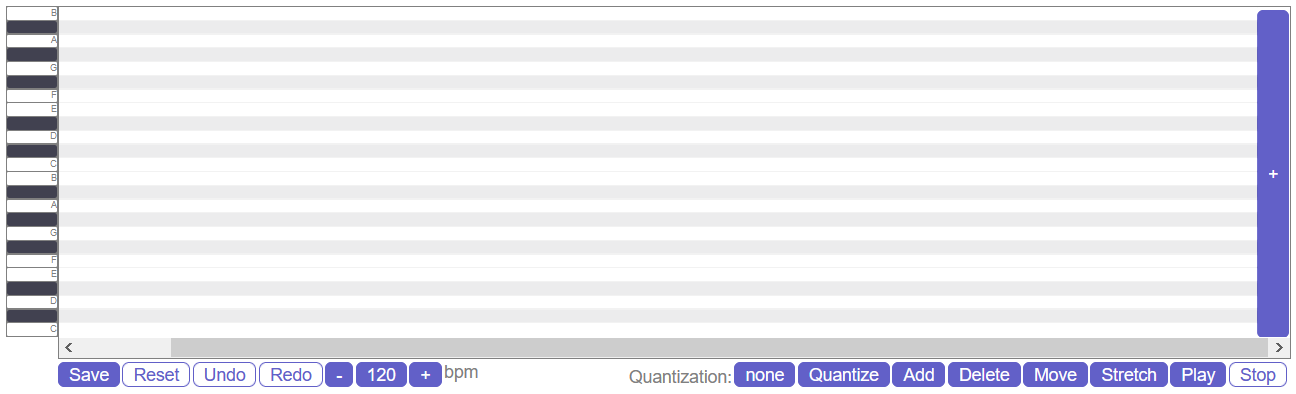
\includegraphics[width=\linewidth]{image/Static.png}
  \caption{A snapshot of the static assets of the DAW, the piano roll is empty}
  \label{fig:static}
\end{figure}

\subsection{Testing}

\blindtext

\subsection{Evaluation}

\blindtext
